%%%%%%%%%%%%%%%%%%%%%%%%%%%%%%%%%%%%%%%%%%%%%%%%%%%%%%%%%%%%%%%%%%%%%%%%%%%%%%%%%%%%%%%%%%%%%%%%%%%%%%%%%%%%%%%%%%%%%%%%%%%%%%%%%%%%%%%%%%%%%%%%%%%%%%%%%%%
% This is just an example/guide for you to refer to when producing your supplementary material for your Frontiers article.                                 %
%%%%%%%%%%%%%%%%%%%%%%%%%%%%%%%%%%%%%%%%%%%%%%%%%%%%%%%%%%%%%%%%%%%%%%%%%%%%%%%%%%%%%%%%%%%%%%%%%%%%%%%%%%%%%%%%%%%%%%%%%%%%%%%%%%%%%%%%%%%%%%%%%%%%%%%%%%%

%%% Version 2.5 Generated 2018/06/15 %%%
%%% You will need to have the following packages installed: datetime, fmtcount, etoolbox, fcprefix, which are normally inlcuded in WinEdt. %%%
%%% In http://www.ctan.org/ you can find the packages and how to install them, if necessary. %%%
%%%  NB logo1.jpg is required in the path in order to correctly compile front page header %%%

\documentclass[utf8]{frontiers_suppmat} % for all articles
\usepackage{url,hyperref,lineno,microtype}
\usepackage[onehalfspacing]{setspace}



% Leave a blank line between paragraphs instead of using \\

\begin{document}
\onecolumn
\firstpage{1}

\title {{\helveticaitalic{Supplementary Material}}}


\maketitle






\begin{figure}[htbp]
\begin{center}
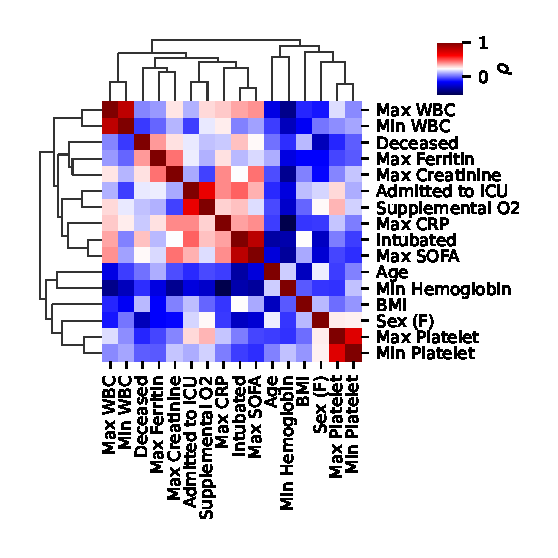
\includegraphics[width=9cm]{FigureS1}% This is a *.eps file
\end{center}
\caption{Correlation map showing Pearson correlation coefficients ($\rho$) between the clinical variables examined.}\label{fig:1}
\end{figure}


\begin{figure}[htbp]
\begin{center}
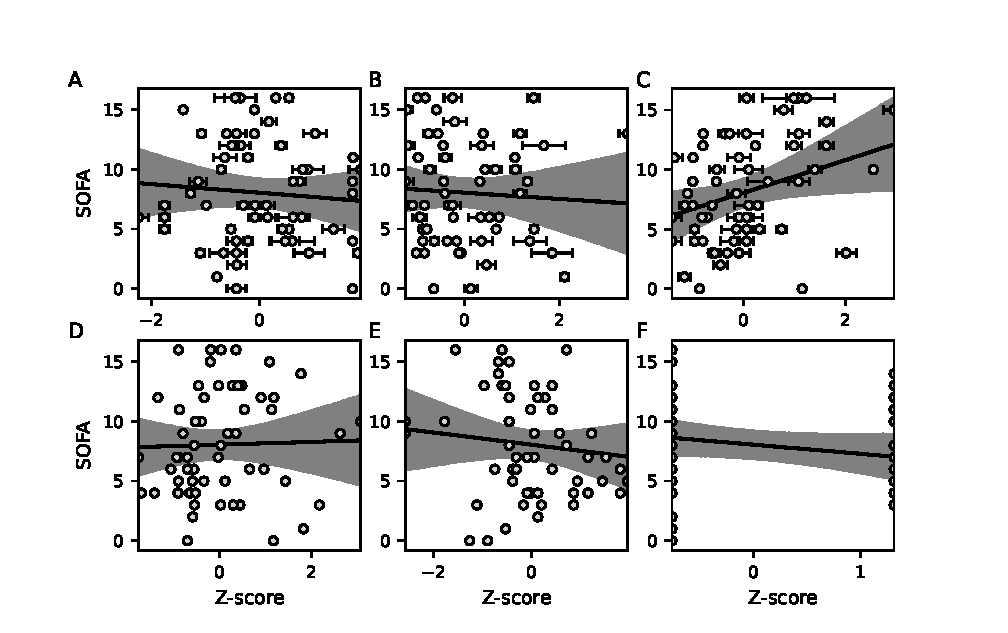
\includegraphics[width=10cm]{FigureS2}
\end{center}
\caption{Scatter plots showing results of multiple linear regression predicting patient SOFA score. Regressors include total predicted (A) HLA-A, (B), HLA-B, and (C) HLA-C binding interactions for each patient toward their corresponding SARS-CoV-2 peptidome. Patient (D) age, (E) BMI, and (F) sex are also included as regressors in the analysis., Error bars represent standard deviation in the independent variable across binding probability thresholds.}\label{fig:2}
\end{figure}

\begin{figure}[htbp]
\begin{center}
\includegraphics[width=10cm]{FigureS3}
\end{center}
\caption{Dose dependence of HLA-C allele subtypes with respect to patient SOFA score. (A-B) Violin plots showing dependence of patient SOFA score on number of alleles in each of the two HLA-C KIR clusters. (C) Bar graph showing the correspondence of the sequence-based clusters identified in the present study to the previously determined KIR clusters. (D-F). Violin plots showing the dependence of patient SOFA score on number of HLA-C alleles from each of the three sequence-based clusters. }\label{fig:3}
\end{figure}

%%% If you are submitting a figure with subfigures please combine these into one image file with part labels integrated.
%%% If you don't add the figures in the LaTeX files, please upload them when submitting the article.
%%% Frontiers will add the figures at the end of the provisional pdf automatically
%%% The use of LaTeX coding to draw Diagrams/Figures/Structures should be avoided. They should be external callouts including graphics.


%\bibliographystyle{frontiersinSCNS_ENG_HUMS} %  for Science, Engineering and Humanities and Social Sciences articles, for Humanities and Social Sciences articles please include page numbers in the in-text citations
%\bibliographystyle{frontiersinHLTH&FPHY} % for Health and Physics articles
%\bibliography{test}

\end{document}
